\chapter{Test of Language Performance} % (fold)
\label{cha:test_of_language}
In order to evaluate the capabilities of \gls{gamble} a test is performed. 
As performance of mathematical operations is in focus, the project group has chosen to only test the language by comparing the execution time of using the \acrshort{gpu} with the execution time of using the \acrshort{cpu} sequentially. \todo{Vi har ingen test af korekthed? -- Troels}

Previously C code for the \acrshort{cpu} has been compared to CUDA C code, both code examples written by the project group, running on the \acrshort{gpu}, see \myref{sub:gpubenchmark}.\todo{er handwritten ikke et fjollet udtryk? MP - Jo, meget, det jo nærmest en gem - Marc}
The results of this test can within reason be expected to have a similar output, meaning that at low data sizes the \acrshort{cpu} is faster than the \acrshort{gpu}, however as the size of the data gets bigger the \acrshort{gpu} is faster.
The reason for the \acrshort{gpu} being slow for low data sizes is that memory needs to be allocated on the \acrshort{gpu}, the input data must be copied to the \acrshort{gpu}, the calculation must be done, and then the data can be copied back to main memory. \todo{Er det nødvendigt at forklarer dette igen? MP - er enig, vi har efterhånden skrevet dette i hvert kapitel - Marc, og ved vi at det er den eneste cost grund? -- Troels}
Once in main memory the data can be further processed e.g. written to a file. 
This means that a relatively high amount of time will not be used for calculations, but for moving data back and forth from main memory to the memory of the \acrshort{gpu}.
The hypothesis from the previous test in \myref{sub:gpubenchmark} was that a more computation heavy test would be faster on the \acrshort{gpu} starting on smaller sizes, so the intersection of the two lines would be for a smaller value on the x-axis. 
The reason for this hypothesis is that because of the large overhead cost the more computations done with the data once it is available in the \acrshort{gpu} will increase the speed of execution compared to the sequential implementation on a \acrshort{cpu}.

It is to be noted that neither the code for the \acrshort{cpu} nor the \acrshort{gpu} has undergone any sort of optimisation process by anything other than the gcc-compiler, as explained in \myref{ssub:makefile}. 
This means that the code could be made faster at execution time, for example by loop-unrolling, multi-core use with threading etc. for the \acrshort{cpu}, and by varying the size of the work group, offline kernel compilation, advanced memory use i.e. local and private memory, for the \acrshort{gpu}.  

\section{The Test} % (fold)
\label{sec:the_test}
The performed test is a simple matrix multiplication with non square matrices.
For the \acrshort{gpu} the built-in matrix operation in \gls{gamble} for matrix multiplication is used. 
The syntax for this operation is: \texttt{matrixA * matrixB}. 
This construction is compiled to a kernel which is invoked for each index in the result matrix, the kernels each calculate just one index of the resulting matrix, and has an inner loop of the size of the columns of the first matrix, which is equal to the rows of the second matrix.
To replicate this for the \acrshort{cpu}, a construct with three nested for-loops is used, where the inner most loop is similar to the one found in the dedicated kernel, and the two outer loops are used to execute the inner loop for each index in the resulting matrix.
Hence the \acrshort{cpu} and \acrshort{gpu} targeted code does the same number of calculations.
 
As an example; for square matrices of size $n$ as input, the amount of calculations is $2*n^3 = O(n^3)$ operations. 
And there are $3*n^2 = O(n^2)$ numbers in the matrices which will be operated on, $2/3$ will be read from and $1/3$ will be written to.\todo{syntes det er lidt lydder lidt kludret - Marc}

When testing execution time, especially on \acrshort{cpu} intensive programs, there is a lot of different variables in the equation. 
The scheduler of the operating system and IO-requests can slow down the execution while caching and cache hits can speed up the computations because of faster memory access. 
These factors will in this test be regarded as the benefits and disadvantages that follows when using the \acrshort{cpu} for compute intensive tasks.
Because of this, trend lines will be used to visualise the data points along with the raw plots.\todo{? MP - Der er da ikke brugt nogle trend lines i vores diagram - Marc}

\subsection{Test Environment} % (fold)
\label{sub:test_environment}
The test for the \acrshort{cpu} is written in C, and the \acrshort{gpu} test is of course written in \gls{gamble}.
As previously mentioned the \acrshort{gpu} test will be using the built-in matrix multiplication of \gls{gamble}, and the \acrshort{cpu} test will be using the three nested for-loops.
The sizes of the matrices are changed using a script which starts the programs where the matrices are given different dimensions and the time result is appended to a file.

The test will be executed on a machine running Ubuntu 14.04.2 LTS, with an Intel Core i5-4670K overclocked to 4.5 GHz as the \acrshort{cpu} and an AMD R9 280x with 3GB of GDDR5 ram and a clock of 1070 MHz as the \acrshort{gpu}.
For main memory 8 GB of DDR3 ram is available.
For running the test on a range of different matrix sizes, a bash script will be used to alter the dimensions through the previously mentioned text files, which will then be loaded by the programs as matrices.
Source code for both programs along with the script used for testing, can be found in \todo{tilføj til apen(dicks)}.

\subsection{Results} % (fold)
\label{sub:results}
After running the test and visualising the execution time for the different matrix sizes, it is clear that the \acrshort{gpu} performs better than the \acrshort{cpu}.
In the graph on \myref{fig:test_results}, we see that the line representing the \acrshort{gpu} is located well below the line representing the \acrshort{cpu}.   
\begin{figure}[h]
    \centering
    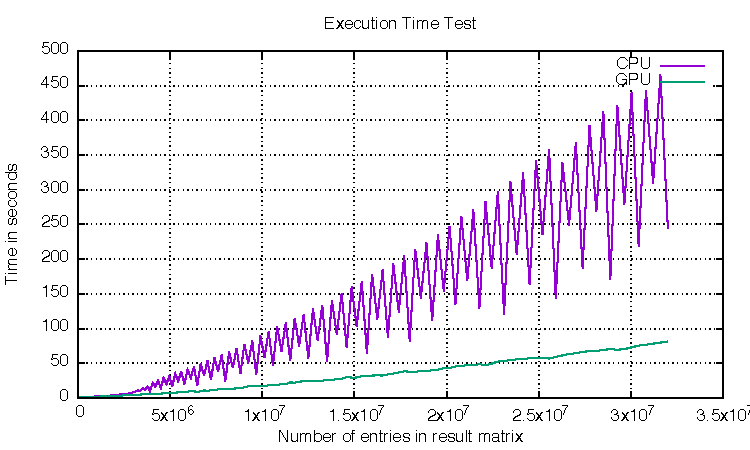
\includegraphics{figures/tests/graph.pdf}
    \caption{Execution time of matrix multiplication, with sequential \acrshort{cpu} and heterogeneous \acrshort{gpu} approach. \todo[inline]{Hvis det kun er på en GPU så er det vel ikke heterogeneous? -- Troels}}\label{fig:test_results}
\end{figure} 
It should however be noted that in the beginning of the graph (the leftmost side), the two lines are very close to each other since time measurements are less precise at such low numbers, and the overhead of initialising and allocating memory for the matrices can well exceed the raw computation time of the multiplication. \todo{Hvis der læses fra harddisken er dette nok en stor faktor. -- Troels}
Be that as is may, the \acrshort{gpu} is always faster in execution time at performing matrix multiplication compared to the \acrshort{cpu} especially when the number of entries in the result matrix exceeds $5*10^6$.
If doing other operations like adding or multiplying a scalar, the results might have been different and looked more like the results from \myref{sub:gpubenchmark}. \todo{Måske noget om at jo flere beregninger der er relativt til andet så vil gamble og gpuen være bedre. -- Troels}

% subsection results (end)
% section the_test (end)

% chapter test_of_language (end) 